\documentclass[acmtog]{acmart}
\usepackage{graphicx}
\usepackage{subfigure}
\usepackage{natbib}
\usepackage{listings}
\usepackage{bm}
\usepackage{amsmath}

\definecolor{blve}{rgb}{0.3372549 , 0.61176471, 0.83921569}
\definecolor{gr33n}{rgb}{0.29019608, 0.7372549, 0.64705882}
\makeatletter
\lst@InstallKeywords k{class}{classstyle}\slshape{classstyle}{}ld
\makeatother
\lstset{language=C++,
	basicstyle=\ttfamily,
	keywordstyle=\color{blve}\ttfamily,
	stringstyle=\color{red}\ttfamily,
	commentstyle=\color{magenta}\ttfamily,
	morecomment=[l][\color{magenta}]{\#},
	classstyle = \bfseries\color{gr33n}, 
	tabsize=2
}
\lstset{basicstyle=\ttfamily}

% Title portion
\title{Assignment 2:\\ {Geometric Modeling}} 

\author{Name:\quad Tian Haoyuan  \\ student number:\ 2020533013
\\email:\quad tianhy@shanghaitech.edu.cn}

% Document starts
\begin{document}
\maketitle

\vspace*{2 ex}

\section{Introduction}
\begin{itemize}
\item Task1 Evaluating points on Bézier curve with De Casteljau's Algorithm has been done.
\item Task2 Constructing the Bézier surface has been done.
\item Task3 Rendering the Bézier surfaces has been done.
\item Task4 Tea party! Patching together multiple Bézier surfaces has been done.
\item Bonus2 B-Spline / NURBS surface construction has been done.
\end{itemize}
\section{Implementation Details}
\begin{enumerate}
	\item \textbf{Task1 Evaluating points on Bézier curve with De Casteljau's Algorithm}\\
	It is not complicated to implement De Casteljau's Algorithm to evaluate Bezier curve. Consider the initial vertices as $P_{0,0}$ to $P_{0,n}$, by cacluating n layers, implementing 
	$$P_{i,j} = (1-t)*P_{i-1,j-1} + t*P_{i,j-1}.$$ Then $P_{n,0}$ would be the position we want, and the vector from $P_{n-1,0}$ to $P_{n-1,1}$ should be the tangent.
	\item \textbf{Task2 Constructing the Bézier surface}\\
	Consider the Bezier surface as interwoven Bezier curves, and I would like to reduce the surface into a curve, so that I can find the point.
	First, implement Bezier curve evaluation with one parameter to one dimension of the 2-D control points, thus returning a single dimension control point vector. Then 
	implement Bezier curve evaluation to this vector with another parameter, we can get the position of the Vertex, as well as one tengent.
	Implement the above steps to the double dimension control point vector again with reverse order, this time we would get another tangent of the Vertex.
	Finally we can get the normal of the Vertex by crossing the two tangents. 
	\item \textbf{Task3 Rendering the Bézier surfaces}\\
	In this task, we have to transform Bezier surfaces to Object class, so that I can draw the mesh.\\
	After implement the evaluation of Bezier surfaces, I am able to get any point I want on the surfaces. I taks an average frequence FREQ to sample the surface, u and v from 0 to 1. For each unit square, I see it as two triangles and push the vertex points into vertices of the targeted object, as well as the corresponding indices.\\
	Now I have the object which can be drawn easily. Beforing drawing the object, implement the read() function that reads from a .bzs file. In the Object class, I initialize VAO, VBO, EBO and several variables, and implement
	drawelement and drawarray function, which is very similar to project Mesh class.
	\begin{figure}[h]
		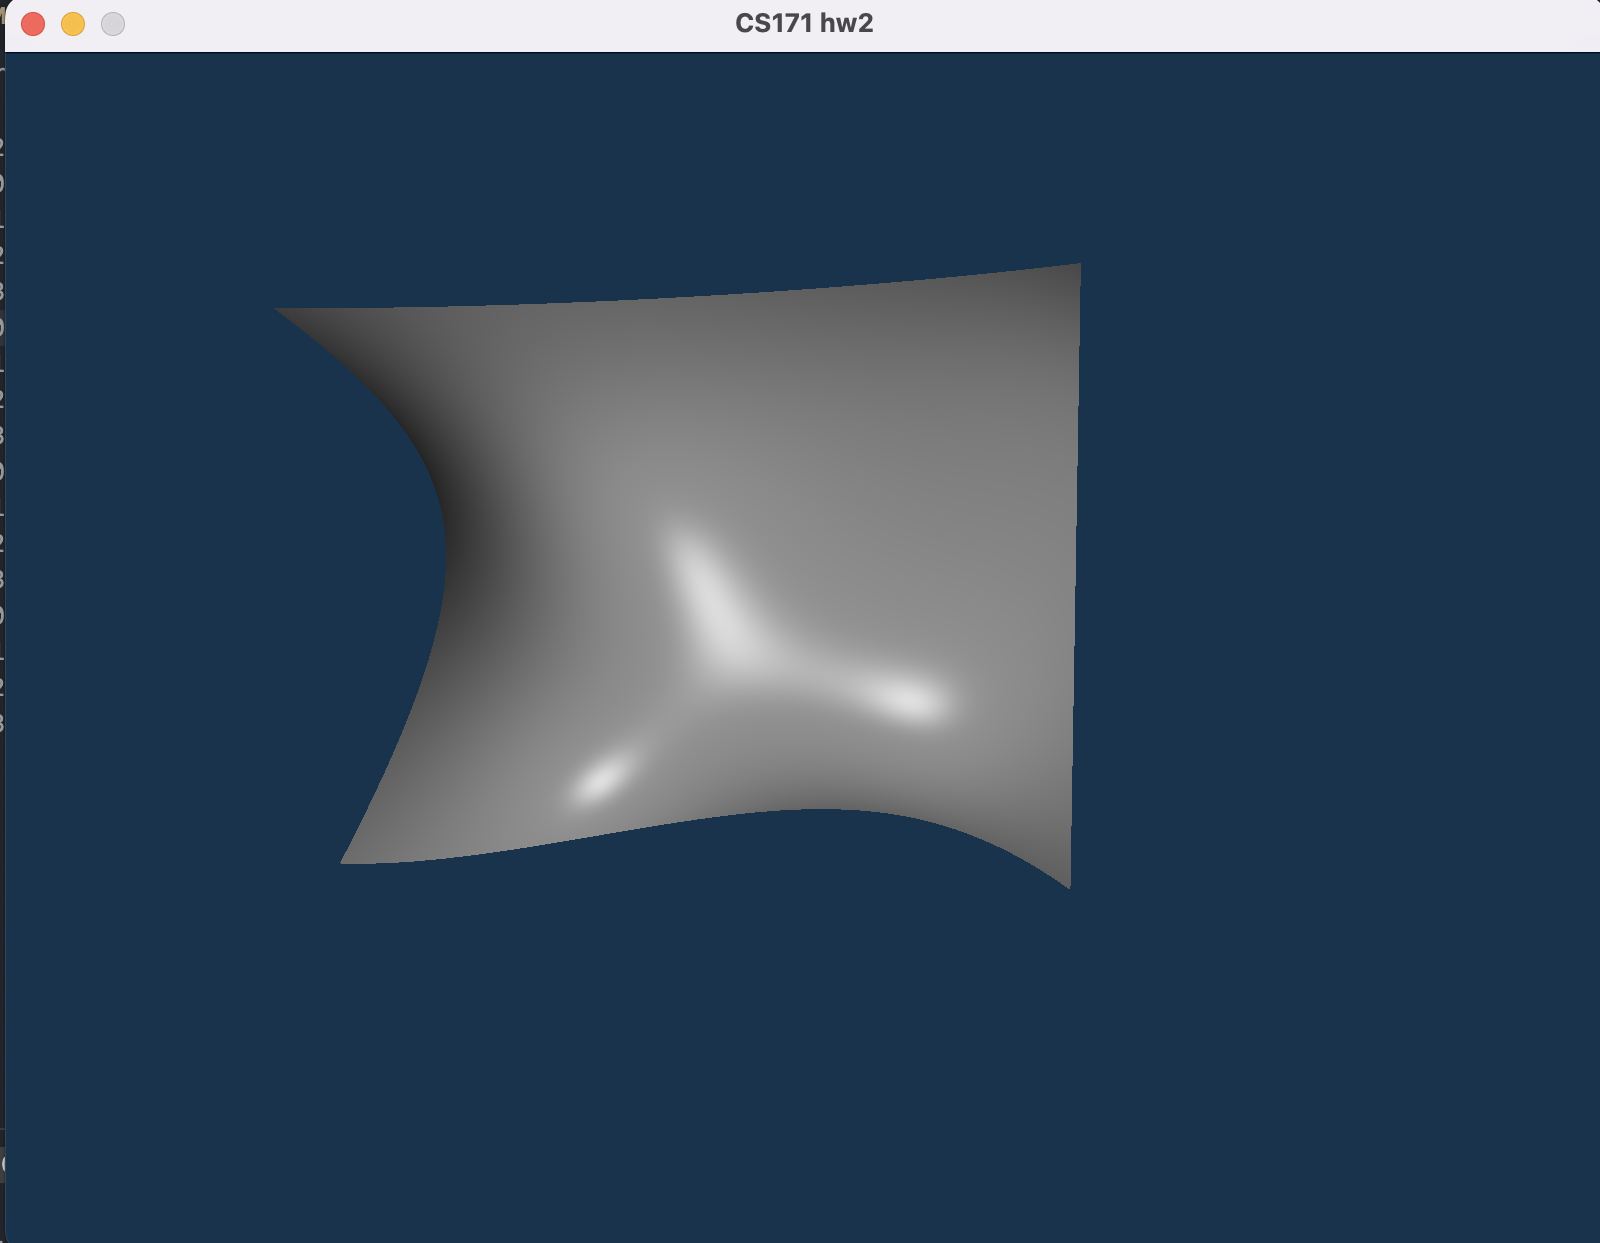
\includegraphics[width=4cm,height=4cm]{bezier.png}
		\caption{Bezier surface}
	\end{figure}
	\item \textbf{Task4 Tea party! Patching together multiple Bézier surfaces}\\
	After the last task, I am able to draw a single Bezier surface. 1st order continuity is guaranteed in files such as tea.bzs, the mission I have to do is to draw multiple continuous surfaces in a single scene.\\
	This is done by iteratively read data of control points in .bzs file and view all triangle meshs as a single object, and render them using the single shader program. The result is as follows.\\
	\begin{figure}[h]
		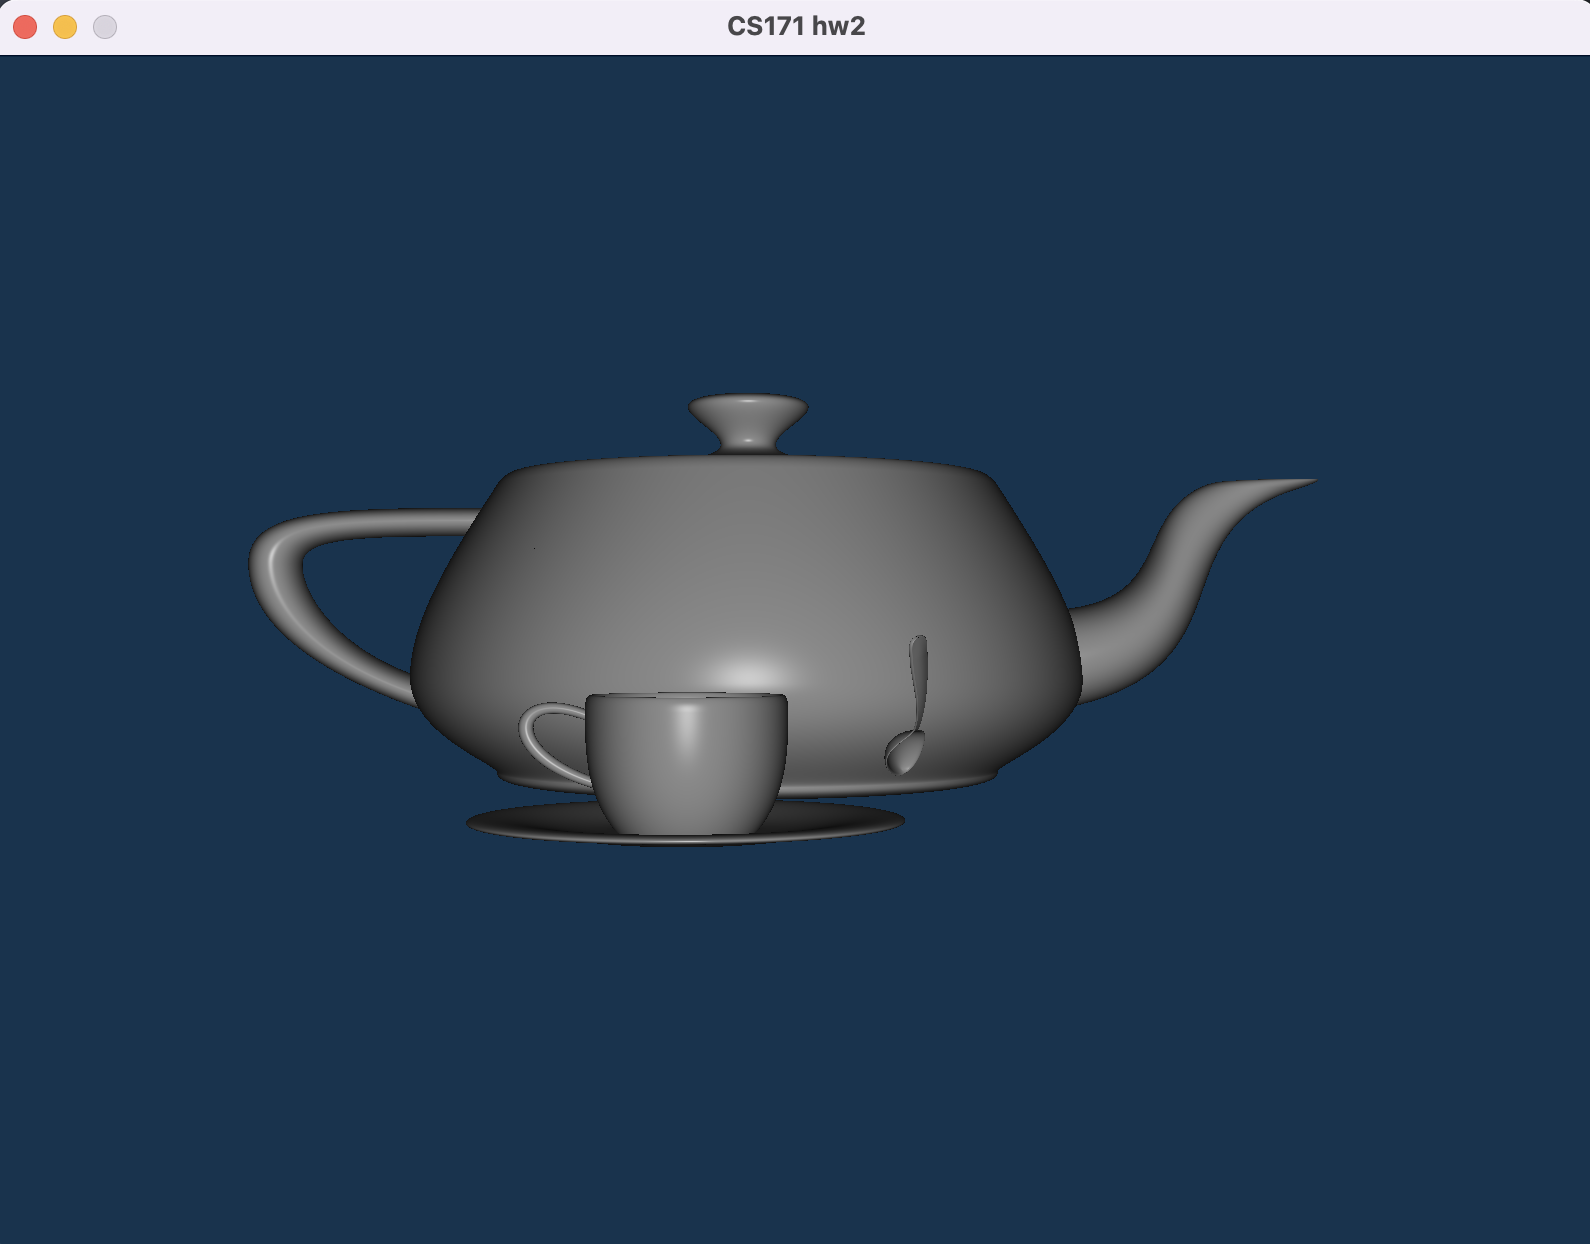
\includegraphics[width=4cm,height=4cm]{teaparty.png}
		\caption{Tea party}
	\end{figure}
	\item \textbf{Bonus2 B-Spline / NURBS surface construction}\\
	B-Spline can avoid several disadvantages of Bezier. As for a Bezier curve, if I want to bend it at some place, then I would taking adding a control point near by my desired change. However, in this way, the order of the whole Bezier curve would be changed, since the evaluation of all points on a Bezier curve takes all control points into consideration.
	Another disadvantage is that, once I want to slightly change a period of the curve, the movememt of a single control should also influence other segement of the curve to some extend.\\
	These make it difficult for a single Bezier surface to simulate a rather normal thing.\\
	While here comes B-Spline, it should only taking neighbor control points into consideration, so that a slight change of a far-away control point would not influence other segement of the curve when evaluating. So drawing the curve or surface can be more independent and intuitive, in terms of being dependent on other segement.\\
	The algorithm to evaluate B-Spline curve resembles that of a Bezier curve. The difference is that we have to determine a series of knots, which should be distributed on the curve, with a total number of m+k+1, where m is the number of control points and k is the order of the curve. The degree is defined be how many control points are taken into consideration when evaluating a point, plus 1.\\
	I distributed the knots in a almost-uniform form, where first degree+1 are assigned to zero, and also last degree+1 are assigned to 1, knots in the middle are uniformally distributed.\\
	Then we can use the knots and degree to evaluate a point with the following function, by de Boor algorithm, 
	% $$N_{i,k}(t) = \frac{t-t_{i}}{t_{i+k-1}-t_i}N_{i,k-1} + \frac{t_{i+k}-t}{t_{i+k-1}-t_i}N_{i,k-1}.$$
	$$P_{i,j} = (1-a_{i,j})*P_{i-1,j-1} + a_{i,j}*P_{i,j-1},$$ with 
	$$a_{i,j} = \frac{\hat{t}-t_i}{t_{i+k-j}-t_i},$$ $\hat{t}$ here is the evaluation parameter from 0 to 1.\\
	It is obvious that the formular used here quite resembles that is used in evaluation of a Bezier curve, dispite the difference of the coefficient. As for coding, I have to consider replacing the original coefficient, and ensurig its dependency as well.\\
	Others are the same as the construction of Bezier surface.\\
	Since the case tea.bzs has only 4 control points per curve, the performance of Bezier and B-Spline should look almost the same.
	A test case I've created to test the different performance of Bezier and B-Spline, 
	\begin{figure}[h]
		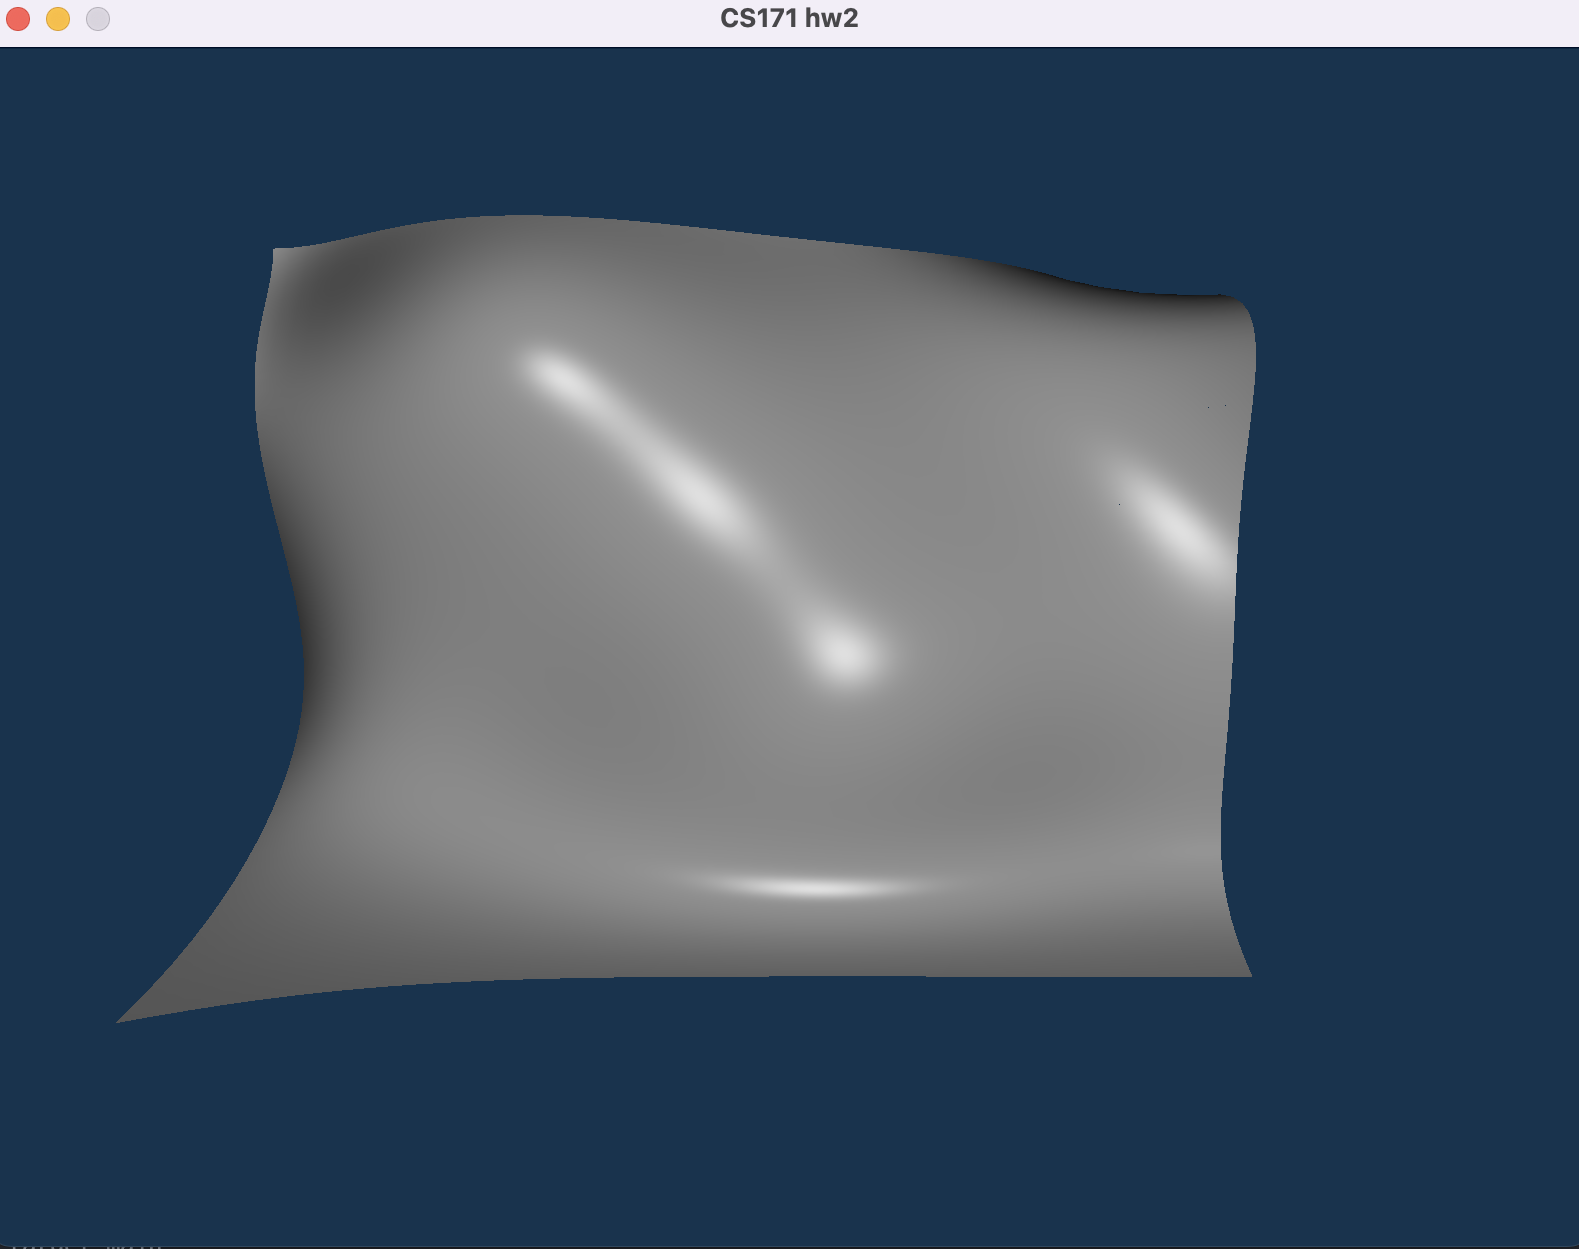
\includegraphics[width=4cm,height=4cm]{using_bezier.png}
		\caption{using Bezier}
	\end{figure}
	Above is the surface constructed by Bezier, followed by the surface constructed by B-Spline, with the same input.\\
	\begin{figure}[h]
		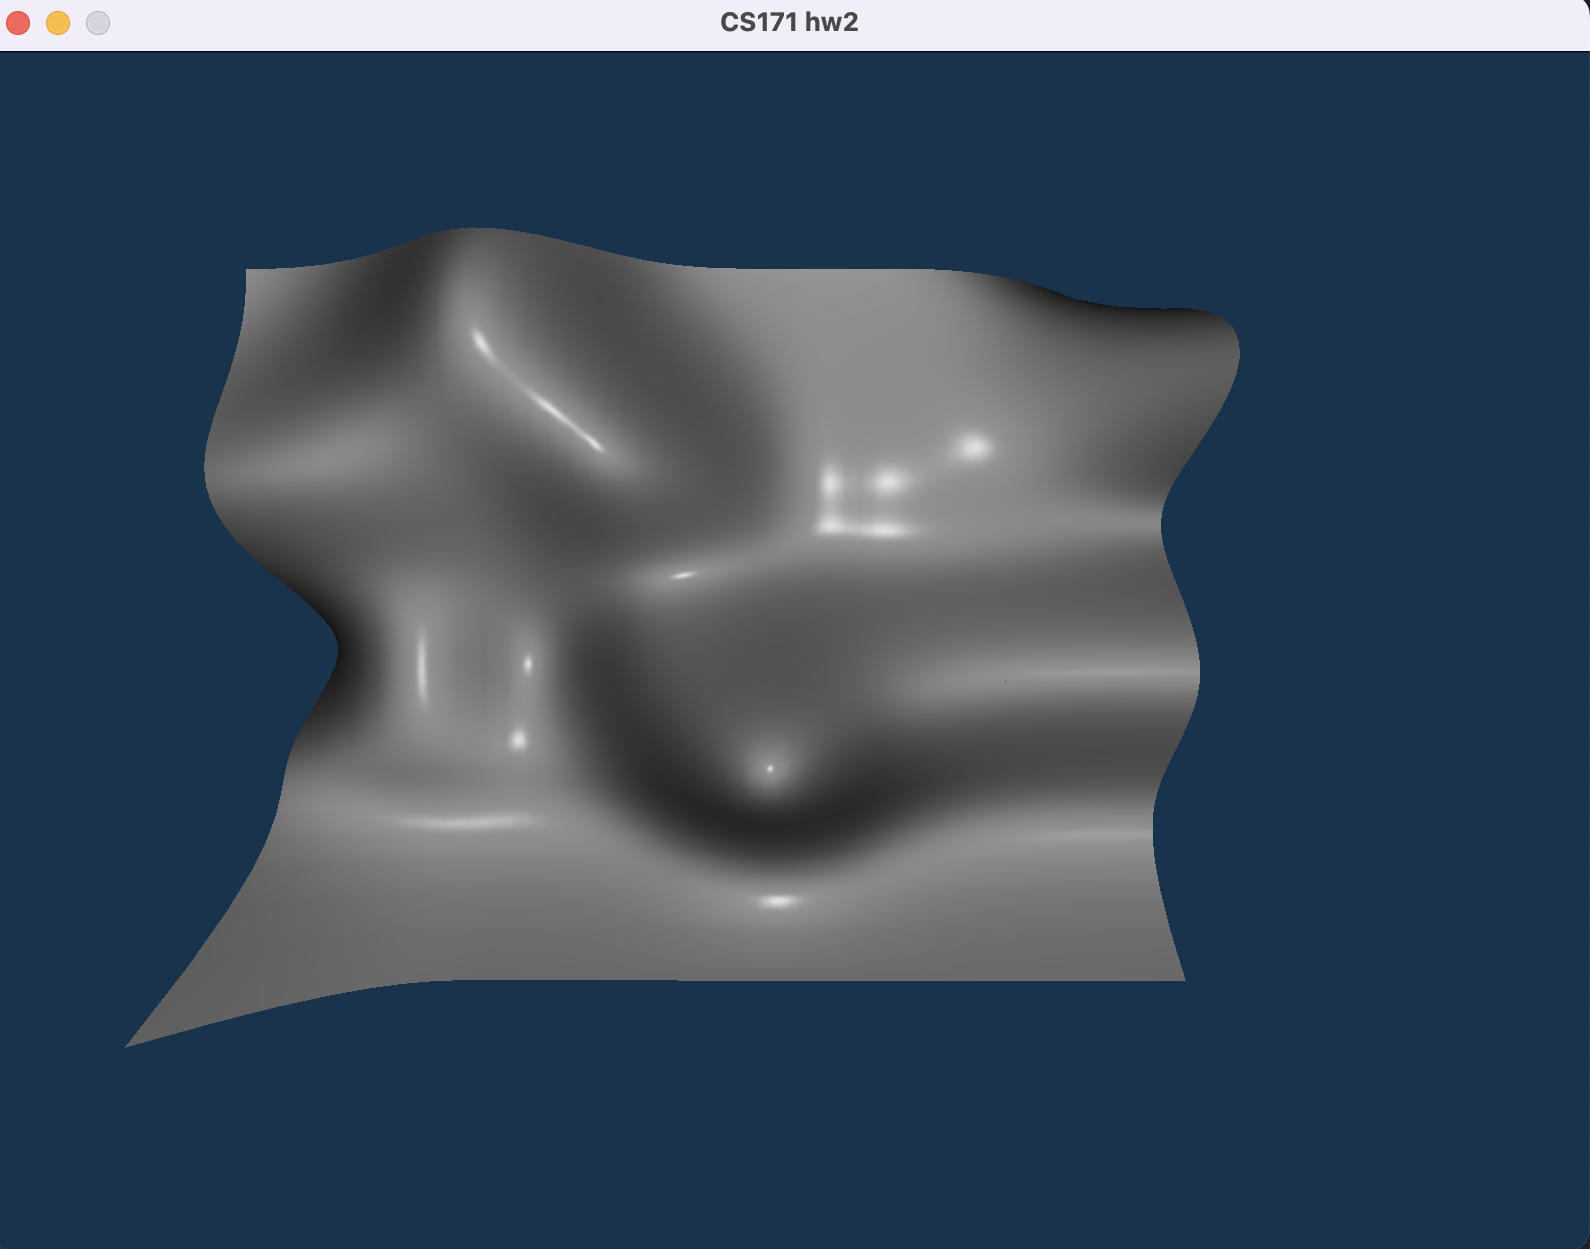
\includegraphics[width=4cm,height=4cm]{using_bspline.png}
		\caption{using B-Spline}
	\end{figure}
	It is obvious that the twists and turns of the surface constructed by B-Spline is steeper. In other words, the .bzs ("../assets/my\_bs.bzs") should naturally be like the version of B-Spline, and the 8 order Bezier can's show the landscape of a surface properly.
\end{enumerate}
\section{Results}
% pictures should be in
After make direction "build" in homepath, you can use cammand "./\_build.sh" to see the result. Pictures are shown above between words as results.
\end{document}
